% \subsection*{Frank-Wolfe}
% \textbf{Definition.} A function $f$ has Lipschitz continuous gradient if:
% \begin{equation*}
%     \forall x,y \in dom(f), \exists L >0 \quad\textit{such that}\quad ||\nabla
%     f(x) -\nabla f(y)||^2 \leq L||x - y||^2
% \end{equation*}

% \begin{theorem}
%   If a convex function $f$ on $C$ has Lipschitz gradient, i.e $||\nabla f(x)-
% \nabla f(y)||_{p}\leq L_{q}||x- y||_{p},\quad\forall x,y\in C$, then
% \begin{equation}
%       &C_{f}\leq L_{q}.\text{diam}_{p}^{2}(C)
% \end{equation}
% \end{theorem}

% \begin{proof}
% $f$ has Lipschitz gradient therefore by the fundamental descent lemma we have,
% \begin{align}
%       &f(y)- f(x)- \langle y- x, \nabla f(x)\rangle \leq \frac{L_{q}}{2}||y- x||_{p}^{2}\\
%       &C_{f} \leq \underset{\underset{x,s,y\in C}{y=(1-\gamma)x+\gamma
% s}}{max}\frac{2}{\gamma^{2}}\frac{L_{q}}{2}\underbrace{||y-
% x||_{p}^{2}}_{=\gamma^{2}||x- s||_{p}^{2}}\\ &C_{f} \leq
% L_{q}\quad\underbrace{\underset{x,s\in C}{max}||x-
% s||_{p}^{2}}_{\overset{\Delta}{=}\textit{diam}_{p}^{2}(C)}\quad\quad\Box.
% \end{align}
% Therefore, assuming $\delta=0$, we get the following optimality certificate

% \begin{align}
%       &f(\alpha^{k})- f^{*}\leq g(\alpha^{k})\leq 2\beta\frac{C_{f}}{t+2}\leq
% 2\beta\frac{L_{q}.\text{diam}_{p}^{2}(C)}{t+2}
% \end{align}
% Thus, we see that the Frank-Wolfe algorithm has a sublinear convergence rate.
% \subsubsection*{Optimality in terms of sparsity of the iterates}
% \textbf{Lemma.} For $f(x)= ||x||_{2}^{2}$ and $1\leq k\leq n$, it holds that

% \begin{aligned}
%       &\textit{min}_{\underset{card(x)\leq
%       k}{x\in\Delta_{n}}}f(x)= \frac{1}{k},\quad\textit{and}\\
%       &g(x)\geq \frac{2}{k}\quad\forall x\in\Delta_{n}\quad\textit{s.t.}\quad card(x)\leq k.
% \end{aligned}
% \end{equation*}
% By the first equality we have, for any vector $x$ s.t. $card(x)= k$, we get $g(x)\leq \frac{1}{k}- \frac{1}{n}$.
% Thus, combining the upper and lower bound, we have that the sparsity (number of used atoms) by the Frank-Wolfe algorithm is worst case optimal.


% As in coordinate descent, we minimize the objective function one coordinate
% (block) at a time. At each iteration, BCFW picks the $i^{th}$ block (from $n$)
% uniformly at random and updates the $i^{th}$ coordinate of the corresponding
% weight, by calling the maximization oracle on the chosen block.
% % \begin{algorithm}[tb]
% %    \caption{Block-Coordinate Frank-Wolfe}
% %    \label{alg:example}
% \begin{algorithmic}
%     \STATE {Let $w^{0}= w_{i}^{0}= \overline{w}^{0}= 0$, $l^{0}= l_{i}^{0}= 0$}\\
%     \FOR {$k=0...K$}{
%         \STATE{Pick $i$ at random in $\{1,...,n\}$}\\
%         \STATE {Solve $y_{i}^{*}=\underset{y_{i}\in\mathcal{Y}_{i}}{\textit{max}}\quad H_{i}(y,w^{k})$}\\
%         \STATE {Let $w_{s}= \frac{1}{n\lambda}\psi_{i}(y_{i}^{*})$, and $l_{s}= \frac{1}{n}L_{i}(y_{i}^{*})$}\\
%         \STATE {Let $\gamma= \frac{\lambda(w_{i}^{k}-w_{s})^{T}w^{k}- l_{i}^{k}+ l_{s}}{\lambda||w_{i}^{k}-w_{s}||^{2}}$, and clip to $[0,1]$}\\
%         \STATE {Update $w_{i}^{k+1}= (1-\gamma)w_{i}^{k}+ \gamma w_{s}$, and $l_{i}^{k+1}= (1-\gamma)l_{i}^{k}+ \gamma l_{s}$}\\
%         \STATE {Update $w^{k+1}= w^{k}+ w_{i}^{k+1}- w_{i}^{k}$, and $l_{i}^{k+1}= (1-\gamma)l_{i}^{k}+ \gamma l_{s}$}\\
%     }
%     \ENDFOR
% \end{algorithmic}
% %\end{algorithm}
% \subsubsection*{Convergence Results}
% \textbf{Definition.} Over each coordinate block $\mathcal{M}^{i}$, let the curvature be given by,

% \begin{align}
%     &C^{(i)}_{f}=
% \underset{\underset{\underset{\gamma\in[0,1]}{y=x+\gamma(s_{[i]}-x_{[i]})}}{x\in\mathcal{M},s_{i}\in\mathcal{M}^{i}}}{sup}\frac{2}{\gamma^{2}}\Big(f(y)-
% f(x)- \langle y_{i}-x_{i}, \nabla_{i} f(x)\rangle\Big)
% \end{aligned}
% \end{equation*}
% Where $x_{[i]}$ refers to the zero-padding of $i^{th}$ coordinate of $x$. And
% let the global \emph{product curvature constant} be,

% \begin{aligned}
%     &C^{\otimes}_{f}= \sum_{i=1}^{n}C^{(i)}_{f}
% \end{aligned}
% \end{equation*}
% \textbf{Theorem.} For the dual structural SVM objective function over the domain
% $\mathcal{M}= \Delta_{|\mathcal{Y}_{1}|}\times...
% \times\Delta_{|\mathcal{Y}_{n}|}$, the total curvature constant
% $C^{\otimes}_{f}$, on the product domain $\mathcal{M}$, is upper bounded by,

% \begin{aligned}
%     &C^{\otimes}_{f} \leq \frac{4R^{2}}{\lambda n}
%     \quad\textit{where} \quad R= \underset{i\in[n], y\in\mathcal{Y}_{i}}{max}||\psi_{i}(y)||_{2}
% \end{aligned}
% \end{equation*}
% \textbf{\textit{Proof.}} By the second order convexity condition on $f$ at $y$, we have
% \begin{align*}
%     f(y)\leq f(x)+ \langle y_{i}-x_{i}, \nabla_{i} f(x)\rangle\\
%     + (y- x)^{T}\nabla^{2}f(x)(y- x)\\
%     f(y)- f(x)- \langle y_{i}-x_{i}, \nabla_{i} f(x)\rangle\\
%     \leq (y- x)^{T}\nabla^{2}f(x)(y- x)
% \end{align*}

% \begin{aligned}
%     &C^{(i)}_{f}\leq\underset{\underset{\underset{\gamma\in[0,1]}{y=x+\gamma(s_{[i]}-x_{[i]})}}{x\in\mathcal{M},s_{i}\in\mathcal{M}^{i}}}{sup}\Big(f(y)- f(x)- \langle y_{i}-x_{i}, \nabla_{i} f(x)\rangle\Big)\\
%     &\leq \underset{\underset{z\in[x,y]\subseteq\mathcal{M}}{x,y\in\mathcal{M},(y-x)\in\mathcal{M}^{[i]}}}{sup}(y- x)^{T}\nabla^{2}f(z)(y- x)\\
%     &\textit{Moreover } \underset{\underset{z\in[x,y]\subseteq\mathcal{M}}{x,y\in\mathcal{M},(y-x)\in\mathcal{M}^{[i]}}}{sup}(y- x)^{T}\nabla^{2}f(z)(y- x)\\
%     &= \lambda \underset{{x,y\in\mathcal{M},(y-x)\in\mathcal{M}^{[i]}}}{sup}(A(y- x))^{T}\nabla^{2}f(z)(A(y- x))
% \end{aligned}
% \end{equation*}

% \begin{aligned}
%     &C^{(i)}_{f}\leq \lambda \underset{v,w\in A\mathcal{M}^{(i)}}{sup}||v- w||^{2}_{2}\leq \lambda \underset{v\in A\mathcal{M}^{(i)}}{sup}||2v||^{2}_{2}
% \end{aligned}
% \end{equation*}
% Where $\forall v\in A\mathcal{M}^{(i)}$, $v$ is a convex combination of the
% feature vectors corresponding to the possible labelings for the $i^{th}$ example
% of the training data, such that $||v||_{2}\leq\textit{ the longest column of A}=
% \frac{1}{n\lambda}R$. Therefore,

% \begin{aligned}
%     &C^{\otimes}_{f}= \sum_{i=1}^{n}C^{(i)}_{f}\leq
% 4\lambda\sum_{i=1}^{n}\Big(\frac{1}{n\lambda}R\Big)^{2}=
% \frac{4}{n\lambda}R^{2}\quad\Box
% \end{aligned}
% \end{equation*}
% First, we observe that the curvature constant for BCFW is $n$ times smaller than
% that of batch Frank Wolfe which is $\leq \frac{4}{\lambda}R^{2}$. Hence the $n$
% times faster convergence rate of BCFW. \subsubsection*{Tightening the bound}
% \textbf{Definition.} Let $||.||$ be a norm on $\mathbb{R}^{n}$. The associated
% dual norm, denoted $||.||_{*}$ is defined as,
% \begin{align*}
%     ||z||_{*}= \underset{z}{\textit{sup}} \{z^{T}x|\quad||x||\leq1\}
% \end{align*}
% We denote the dual norm of $l_{p}$ by $l_{q}$. For $p=2$ we have $q=2$ and for $p=1$, $q=\infty$.
% \textit{Problem.}\quad For $p= q= 2$ we get $\textit{diam}_{2}^{2}(C)= 2n$, and the Lipschitz constant $L_{q}$ is the largest eigenvalue of the hessian.
% \begin{align*}
%     &\lambda A^{T}A= \frac{1}{n^{2}\lambda}\Big(\langle \psi_{i}(y)-
% \psi_{j}(y\prime) \rangle\Big)_{(i,y),(j,y\prime)}\\ &\textit{And say}\quad
% \langle \psi_{i}(y)- \psi_{j}(y\prime) \rangle \approx 1\quad\textit{for a lot
% of outputs, we get:}\\
%     &\mathbbm{1}^{T}\mathbbm{1}\approx \mathbbm{1}\underbrace{diam_{2}(C)}_{=\sqrt{2n}}
% \end{align*}
% Hence the largest eigenvalue the hessian, and therefore the Lipschitz constant,
% can scale with the dimension of $A^{T}A$, i.e exponentially with the size of the
% training data, rendering the bound above very loose, and thus of little
% practical use. \\

% \textit{Solution.}\quad Taking $p=1$ and therefore $q=\infty$, we get
% $L\textit{diam}^{2}(C)\approx \frac{4}{\lambda}R^{2}$.\\ \\
% Combined with the the convergence results above, we get a sublinear convergence
% rate for BCFW. And although subgradient methods converge at the same rate, BCFW
% presents an adaptive stepsize and an indication as to when to terminate, making
% it a more practical alternative.



% \subsubsection*{Away steps Frank-Wolfe}
% When the minimizer of the objective function lies at the boundary of the domain,
% after a number of iterations, the duality gap starts to stagnate.\\ As a result
% of the strong dependency of the immediate iterate on previously accumulated
% atoms in the active set, as it approaches to boundary, the F-W algorithm starts
% to zig-zag around the descent direction as can be seen in figure 2.\\
% % \begin{algorithm}[tb]
% %    \caption{Away-steps Frank-Wolfe}
% %    \label{alg:example}
% \begin{algorithmic}
%     \STATE {Let $x_{0}\in\mathcal{A}$ and $S_{0}:=\{x_{0}\}$}\\
%     \FOR {$t=0...T$}{
%         \STATE{Let $s_{t}:= LMO_{\mathcal{A}}(\nabla f(x_{t}))$ and $d^{FW}_{t}:= s_{t}- x_{t}$}\\
%         \STATE{Let $v_{t}\in \underset{v\in S_{t}}{\textit{argmax}}\langle\nabla f(x_{t}), v\rangle$ and $d^{A}_{t}:= x_{t}- v_{t}$}\\
%         \STATE {\textbf{if} $g^{FW}_{t}=\langle-\nabla f(x_{t}),
% d^{FW}_{t}\rangle\leq \epsilon$ \textbf{then return} $x_{t}$}\\ \STATE
% {\textbf{if} $\langle-\nabla f(x_{t}), d^{FW}_{t}\rangle\geq \langle-\nabla
% f(x_{t}), d^{A}_{t}\rangle$\quad\textbf{then}}\\
% \STATE{\quad\quad\quad$d_{t}=d^{FW}_{t}$ and $\gamma^{max}=1$}\\
% \STATE{\textbf{else}}\\
%         \STATE{\quad\quad\quad $d_{t}=d^{A}_{t}$ and
% $\gamma^{max}=\frac{\alpha^{(t)}_{v_{t}}}{1-\alpha^{(t)}_{v_{t}}}$}\\
% \STATE{Line-search: $\gamma_{t}\in\underset{\gamma}{argmin}f(x_{t}+\gamma
% d_{t})$}\\ \STATE{Update $x_{t}= x_{t}+\gamma_{t}d_{t}$}\\ } \ENDFOR
% \end{algorithmic}
% %\end{algorithm}
% % \begin{figure}
% %   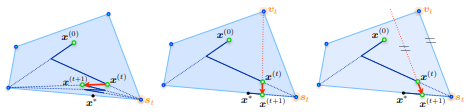
\includegraphics[width=\linewidth]{fig2.png}
% %   \caption{(left) The FW algorithm zig-zags when the solution $x$ lies on the
% % boundary. (middle) Adding the possibility of an away step attenuates this
% % problem. (right) As an alternative, a pairwise FW step.}
% %   \label{fig:Away steps}
% % \end{figure}

% To address this issue an improved variant of F-W named \textbf{Away-steps
% Frank-Wolfe} adds the possibility of moving away (by removing a fraction of) a
% maximizer of the $LMO_{\mathcal{S_{t}}}$ in the active set. While this slows
% down each iteration it should be noted that the added step is easier than
% $LMO_{\mathcal{A}}$ given that we maximize over a subset of $\mathcal{A}$.
% Furthermore, given that this variant converges linearly, the algorithm
% progresses in a fewer number of iterations in the descent direction, making it
% much faster than the original F-W.




% \subsubsection*{Randomized Away-step Frank-Wolfe}
% A crucial assumption in constructing the BCFW is whether the domain is
% block-separable. While this is true in the context of the structured SVM, this
% leaves out important cases such as $l_{1}$ constrained optimization (e.g. lasso
% type problems). \\
% Moreover, while being an improvement on the classical variant by being
% $n=\textit{size of the data}$ times cheaper per iteration, BCFW still converges
% at a sublinear rate unlike the Away-step FW.\\

% \textbf{The Randomized Away-steps Frank-Wolfe (RAWF)} finds a compromise between
% the two variants. By subsampling a $\eta\in(0,1]$ portion of the domain
% $\mathcal{A}$ in the $LMO$ and adding an away step at each iteration, we get a
% linear convergence rate with cheaper oracle calls than that of the original F-W.
% \subsubsection*{Convergence results}
% \textbf{Definition.}
% Let the \textit{away curvature} $C^{A}_{f}$ and the \textit{geometric strong convexity} constants be, respectively
% % 
% % \begin{aligned}
% %     &C^{A}_{f}= \underset{\underset{\underset{\gamma\in[0,1]}{y=x+\gamma(s-
% % x)}}{x,s,v\in\mathcal{M}}}{sup}\frac{2}{\gamma^{2}}\Big(f(y)- f(x)-
% % \gamma\langle \nabla f(x), s- v\rangle\Big)\\ &\mu^{A}_{f}=
% % \underset{x\in\matcal{M}}{\textit{inf}}\underset{\underset{\langle\nabla f(x),
% % x^{*}-x\rangle <
% % 0}{x^{*}\in\mathcal{M}}}{\textit{inf}}\frac{2}{\gamma^{A}(x,x^{*})^{2}}B_{f}(x,x^{*})\\
% % &\texit{where}\quad\gamma^{A}(x,x^{*})=\frac{\langle -\nabla f(x), x^{*}-
% % x\rangle}{\langle -\nabla f(x), s_{f}(x)- v_{f}(x)\rangle}\\
% % \end{aligned}
% % \end{equation*}
% And $s_{f}, v_{f}(x)$ are the FW atom and away atom respectively, starting from $x$.\\

% \textbf{Theorem.} Consider the set $\mathcal{M}=conv(\mathcal{A})$, with
% $\mathcal{A}$ a finite set of extreme atoms, adter $T$ iterations of RAFW, we
% have the following convergence rate
% 
% \begin{aligned}
%     &E\big[f(x_{T+1})\big]- f^{*}\leq \Big(f(x_{0})- f^{*}\Big).\Big(1- \eta^{2}\rho_{f}\Big)^{\textit{max}\{0,\lfloor\frac{T-s}{2}\rfloor\}}
% \end{aligned}
% \end{equation*}
% With $\rho_{f}=
% \frac{\mu^{A}_{f}}{4C^{A}_{f}},\quad\eta\frac{p}{|\mathcal{A}|}\quad$ and
% $\quad s=|S_{0}|$.\\

% \textbf{Proof sketch.} First we upper-bound $h_{t}=f(x_{t})- f^{*}$ by the
% pairwise dual gap $\tilde{g}_{t}=\langle \tilde{s}_{t}- v_{t}\rangle$, then we
% lower bound the progress $h_{t}- h_{t+1}$ by using the away curvature constant
% in similar way to the proof in (Lacoste-Julien \& Jaggi, 2015, Theorem
% 8).$\Box$\\ \\
% With the above theorem, we get
% 
% \begin{aligned}
%     &\underset{t\rightarrow \infty}{\textit{lim}} \frac{E f(x_{t+1})- f^{*}}{E f(x_{t})- f^{*}} \in \big(0,1\big)
% \end{aligned}
% \end{equation*}
% Thus proving a linear convergence rate for the Randomized Away-steps Frank-Wolfe.
% % \begin{algorithm}[tb]
% %    \caption{Randomized Away-steps Frank-Wolfe}
% %    \label{alg:example}
% \begin{algorithmic}
%     \STATE {Let $x_{0}=\sum_{v\in\mathcal{A}}\alpha^{(0)}_{v}$ with $s= |S_{0}|$, a subsampling parameter $1\leq p\leq |\mathcal{A}|$.}\\
%     \FOR {$t=0...T$}{
%         \STATE{Get $\mathcal{A}_{t}$ by sampling $min\{p,|\mathcal{A}\setminus S_{t}|\}$  elements uniformly from $|\mathcal{A}\setminus S_{t}|$}\\
%         \STATE {Compute $s_{t}= LMO(\nabla f(x), S_{t}\bigcup \mathcal{A}_{t})$}\\
%         \STATE {Let $d^{FW}_{t}= s_{t}- x_{t}$\quad\quad\textbf{RFW step}}\\
%         \STATE {Compute $v_{t}= LMO(-\nabla f(x), S_{t})$}\\
%         \STATE {Let $d^{A}_{t}= x_{t}- v_{t}$\quad\quad\quad\textbf{Away step}}\\
%         \STATE {\textbf{if} $\langle-\nabla f(x_{t}), d^{FW}_{t}\rangle\geq \langle-\nabla f(x_{t}), d^{A}_{t}\rangle$\quad\textbf{then}}\\ \STATE{\quad\quad\quad$d_{t}=d^{FW}_{t}$ and $\gamma^{max}=1$}\\
%         \STATE{\textbf{else}}\\
%         \STATE{\quad\quad\quad $d_{t}=d^{A}_{t}$ and $\gamma^{max}=\frac{\alpha^{(t)}_{v_{t}}}{1-\alpha^{(t)}_{v_{t}}}$}\\
%         \STATE{Let $x_{t+1}= x_{t}+ \gamma_{t}d_{t}$}\\
%         \STATE{Let $S_{t+1}= \{v\in\mathcal{A}\quad s.t.\quad \alpha^{(t)}_{v^{}_{t}} > 0$\}}\\
%     }
%     \ENDFOR
% \end{algorithmic}
% %\end{algorithm}

%%% Local Variables:
%%% mode: latex
%%% TeX-master: "mainProject"
%%% End:

% \clearpage
% In \citet{lacoste-julienBlockCoordinateFrankWolfeOptimization2013} 
% We define the \emph{linearize duality gap} for the k'th iterate as:
% \begin{equation}
%   g(\alpha^{k}) \triangleq \max_{s\in\mathcal{M}}\langle \alpha^{k}-s, \nabla f(\alpha^{k})\rangle
%   \label{eq:dualityGapDef}
% \end{equation}
% We
% \begin{align}
%     &f(s)\geq f(\alpha^{k})+ \langle \alpha^{k}-s, \nabla f(\alpha^{k})\rangle\\
%     &\Longrightarrow g(\alpha^{k})=
%       \min_{s\in\mathcal{M}}\langle \alpha^{k}-s, \nabla
%       f(\alpha^{k})\rangle \geq f(\alpha^{k})- f^{*}
% \end{align}
% We can thus see that the duality gap gives us a computable optimality guarantee. \\

% % \begin{definition}
% %   The curvature constant $C_{f}$ is given by the maximum relative deviation of
% %   the objective function f from its linear aaporximations, over the domain
% %   $\mathcal{M}$,
% % \end{definition}


% % \begin{align}
% %     &C_{f}= \underset{\underset{ \gamma\in[0,1],
% % y=x+\gamma(s-x)}{x,s\in\mathcal{M}}}{sup}\frac{2}{\gamma^{2}}\Big(f(y)- f(x)-
% % \langle y-x, \nabla f(x)\rangle\Big)
% % \end{align}
% % Intuitively, the curvature constant can be seen as a measure of how flat the
% % objective function is. For example, if the objective is linear, say $f(x)= ax+
% % b$ and $x\in[e,f]$ then $\nabla f(x)= a$ and the curvature constant is zero:
% % \begin{align}
% %     &C_{f}= \frac{2}{\gamma^{2}}\Big(ay+ b- ax- b +(-ay +ax)\Big)= 0
% % \end{align}
% % Moreover $s=\textit{argmin}_{s\in[e,f]}\langle s, a\rangle= \frac{e}{a}$. Hence
% % we reach the minimum in one F-W step. Thus, we can observe that for flatter
% % functions, that is with smaller curvature constants, Frank-Wolfe should converge
% % faster. 

% % \begin{theorem}
% %   The duality gap obtained in the $t^{th}$ iteraton of the Frank-Wolfe algorithm
% % satisfies
% % \begin{align}
% %     &g(x_{t})\leq 2\beta\frac{C_{f}}{t+2}(1+\delta)
% % \end{align}
% % Where $\beta= \frac{27}{8}$ and $\delta$ is the approximation error tolerated in
% % the $LMO$.
% % \end{theorem}


% %%% Local Variables:
% %%% mode: latex
% %%% TeX-master: "mainProject"
% %%% End: